\documentclass[12pt]{article}
\usepackage[utf8]{inputenc}
\usepackage{polski}
\usepackage{listing}
\usepackage{amsmath}
\usepackage{multicol}
\usepackage{graphicx}
\usepackage{enumitem}
\graphicspath{ {./images/} }
\title{
	Obliczenia naukowe \\
	Sprawozdanie 3
}
\addtolength{\oddsidemargin}{-.8in}
\addtolength{\evensidemargin}{-.8in}
\addtolength{\textwidth}{1.75in}
\addtolength{\topmargin}{-.7in}
\addtolength{\textheight}{1.75in}

\date{23 listopada 2019}
\author{Józef Piechaczek}

\begin{document}

\pagenumbering{gobble}
\maketitle
\newpage
\pagenumbering{arabic}

\setlength{\abovedisplayskip}{5pt}
\setlength{\belowdisplayskip}{5pt}

\section{Zadanie 1}
Zadanie 1 polega na utworzeniu funkcji rozwiązującej równianie $f(x) = 0$ za pomocą metody bisekcji. \textbf{Definicja funkcji:}
\begin{verbatim}
function mbisekcji(f, a::Float64, b::Float64, delta::Float64, 
epsilon::Float64)
\end{verbatim}
\textbf{Dane:}
\begin{itemize}[leftmargin=4.0cm,labelsep=0.4cm]
\item[$f$] funkcja $f(x)$ zadana jako anonimowa funkcja
\item[$a, b$] końce przedziału początkowego
\item[$delta, epsilon$] dokładności obliczeń
\end{itemize}
\textbf{Wyniki:} 
\begin{itemize}[leftmargin=4.0cm,labelsep=0.4cm]
\item[$(r, v, it, err)$] czwórka, gdzie
\item[$r$] przybliżenie pierwiastka równiania 
\item[$v$] wartość $f(r)$
\item[$it$] liczba iteracji
\item[$err$] sygnalizacja błędu\\
0 - brak błędu\\
1 - funkcja nie zmienia znaku w przedziale $[a,b]$
\end{itemize}

\noindent \textbf{Opis metody:}\\
Metoda bisekcji korzysta z twierdzenia Darboux do szacowania wartości pierwiastka funkcji. Twierdzenie to mówi, że funkcja ciągła na danym przedziale $[a, b]$ i zmieniająca znak na tym przedziale (co opisuje nierówność $f(a)f(b) < 0$) posiada miejsce zerowe w $[a,b]$. Metoda w pojedynczej iteracji dzieli podany przedział na połowę, obliczając środek przedziału $c=\frac{1}{2}(b-a)$. Następnie obliczamy wartość funkcji w punkcie c, tj. $f(c)$. Sprawdzamy znak wartości $f(c)$ i rozpatrujemy nowy przedział $(a, c)$ albo $(c, b)$ taki, że funkcja zmienia znak w danym przedziale. Metoda kończy działanie w momencie gdy osiągamy zadaną dokładność, tj. przedział jest dostatecznie niewielki lub wartość w punkcie c jest dostatecznie bliska zeru. Metoda ma zbieżność liniową.
\\
\\
\noindent \textbf{Opis algorytmu:}\\
Aby algorytm był jak najlepszy z numerycznego punktu widzenia wprowadziłem następujące zmiany:
\begin{enumerate}
	\item Środek przedziału liczymy za pomocą wzoru $e=(b-a)/2, c=a+e$. Jest to dokładniejszy sposób niż obliczanie środka klasyczną metodą $c=(a+b)/2$, gdyż klasyczna metoda mogła powodować, iż środek przedziału znajdował się poza przedziałem dla niektórych przypadków.
	\item Wartości funkcji na krańcach przedziału porównujemy za pomocą \texttt{sign(f(c)) != sign(f(a))}, gdyż sprawdzanie tego za pomocą warunku $f(a)f(b) < 0$ mogło powodować overflow lub underflow.
\end{enumerate}
Algorytm kończy pracę na jeden z dwóch sposobów
\begin{enumerate}
\item Gdy zadana dokładność została osiągnięta
\item Gdy funkcja nie zmienia znaku w zadanym przedziale - error code 1
\end{enumerate}





\section{Zadanie 2}
Zadanie 2 polega na utworzeniu funkcji rozwiązującej równianie $f(x) = 0$ za pomocą metody Newtona. \textbf{Definicja funkcji:}
\begin{verbatim}
function mstyczych(f, pf, x0::Float64, delta::Float64, 
epsilon::Float64, maxit::Int)
\end{verbatim}
\textbf{Dane:}
\begin{itemize}[leftmargin=4.0cm,labelsep=0.4cm]
\item[$f, pf$] funkcja $f(x)$ oraz pochodna $f'(x)$ zadane jako anonimowe funkcje
\item[$x0$] przybliżenie początkowe
\item[$delta, epsilon$] dokładności obliczeń
\item[$maxit$] maksymalna liczba iteracji
\end{itemize}
\textbf{Wyniki:} 
\begin{itemize}[leftmargin=4.0cm,labelsep=0.4cm]
\item[$(r, v, it, err)$] czwórka, gdzie
\item[$r$] przybliżenie pierwiastka równiania 
\item[$v$] wartość $f(r)$
\item[$it$] liczba iteracji
\item[$err$] sygnalizacja błędu\\
0 - brak błędu\\
1 - nie osiągnieto wymaganej dokładności w $maxit$ operacji\\
2 - pochodna bliska zeru
\end{itemize}

\noindent \textbf{Opis metody:}\\
Metoda Newtona polega na lokalnej aproksymacji liniowej za pomocą stycznych. W tej metodzie iteracyjnej $x_{n+1}$ jest określone jako odcięta punktu przecięcia z osią x stycznej do krzywej $y=f(x)$ w punkcie $(x_n,f(x_n))$. Zatem kolejne przybliżenia pierwiastka równiania można określić za pomocą wzoru:
\begin{equation*}
x_{n+1}=x_n-\frac{f(x_n)}{f'(x_n)}
\end{equation*}
Metoda Newtona ma zbieżność kwadratową, zatem zbiega szybciej niż metoda bisekcji i siecznych. Wadą tej metody natomiast jest konieczność liczenia pochodnej funkcji. Inna wadą jest fakt, iż zbieżność nie zachodzi zawsze. W wielu przypadkach metoda jest rozbieżna, kiedy punkt startowy znajduje się zbyt daleko od poszukiwanego miejsca zerowego.
\\
\\
\noindent \textbf{Opis algorytmu:}\\
Program może kończyć działanie na jeden z czterech sposobów:
\begin{enumerate}
	\item Gdy spełniona jest wymagana dokładność na początku działania programu, tj. $f(x_0) < epsilon$
	\item Gdy pochodna jest bliska zeru ($|f'(x_0)|<epsilon$) - funkcja zwraca error code 2
	\item Gdy w danej iteracji spełniona jest zadana dokładność ($|x_{n+1}-x_n|<delta$ lub $|f(x_{n+1})|<epsilon$)
	\item Gdy nie osiągnięto zadanej dokładności w $maxit$ iteracji - error code 1
\end{enumerate}





\section{Zadanie 3}
Zadanie 3 polega na utworzeniu funkcji rozwiązującej równianie $f(x) = 0$ za pomocą metody siecznych. \textbf{Definicja funkcji:}
\begin{verbatim}
function msiecznych(f, x0::Float64, x1::Float64, delta::Float64, 
epsilon::Float64, maxit::Int)
\end{verbatim}
\textbf{Dane:}
\begin{itemize}[leftmargin=4.0cm,labelsep=0.4cm]
\item[$f$] funkcja $f(x)$ zadana jako anonimowa funkcja
\item[$x0, x1$] przybliżenia początkowe
\item[$delta, epsilon$] dokładności obliczeń
\item[$maxit$] maksymalna liczba iteracji
\end{itemize}
\textbf{Wyniki:} 
\begin{itemize}[leftmargin=4.0cm,labelsep=0.4cm, itemsep=0.00cm]
\item[$(r, v, it, err)$] czwórka, gdzie
\item[$r$] przybliżenie pierwiastka równiania 
\item[$v$] wartość $f(r)$
\item[$it$] liczba iteracji
\item[$err$] sygnalizacja błędu\\
0 - brak błędu\\
1 - nie osiągnieto wymaganej dokładności w $maxit$ operacji\\
\end{itemize}

\noindent \textbf{Opis metody:}\\
Metoda siecznej jest podobna do metody Newtona, jednak w tej metodzie pochodną zastępujemy ilorazem różnicowym postaci:
\begin{equation*}
f'(x_n) \approx \frac{f(x_n)-f(x_{n-1})}{x_n-x_{n-1}}
\end{equation*}
Otrzymujemy więc następujący wzór rekurencyjny
\begin{equation*}
x_{n+1} = x_n - f(x_n) \frac{x_n-x_{n-1}}{f(x_n)-f(x_{n-1})}, n \geq 1
\end{equation*}
Metoda zatem potrzebuje dwóch punktów startowych. Metoda ta ma zbieżność wynoszącą $\frac{1+\sqrt{5}}{2}$, zatem jest wolniejsza od metody Newtona, ale za to nie wymaga liczenia pochodnej funkcji.
\\
\\
\noindent \textbf{Opis algorytmu:}\\
Algorytm kończy działanie na jeden z dwóch sposobów:
\begin{enumerate}
\item Gdy spełniona jest zadana dokładność
\item Gdy zadana dokładność nie została osiągnięta w $maxit$ iteracji - error code 1
\end{enumerate}

\section{Zadanie 4}
Celem zadania 4 jest wyznaczenie pierwiastków równania $sin x - (\frac{1}{2}x)^2 = 0$ za pomocą zaprogramowanych wcześniej metod:
\begin{enumerate}
	\item bisekcji z przedziałem początkowym $[1.5, 2]$ i $\delta=\frac{1}{2}10^{-5}$, $\epsilon=\frac{1}{2}10^{-5}$ 
	\item Newtona z przybliżeniem początkowym $x_0 = 1.5$ i $\delta=\frac{1}{2}10^{-5}$, $\epsilon=\frac{1}{2}10^{-5}$ 
	\item siecznych z przybliżeniami początkowymi $x_0=1$, $x_1=2$ i $\delta=\frac{1}{2}10^{-5}$, $\epsilon=\frac{1}{2}10^{-5}$ 
\end{enumerate}

\begin{figure}[!h]
	\centering
  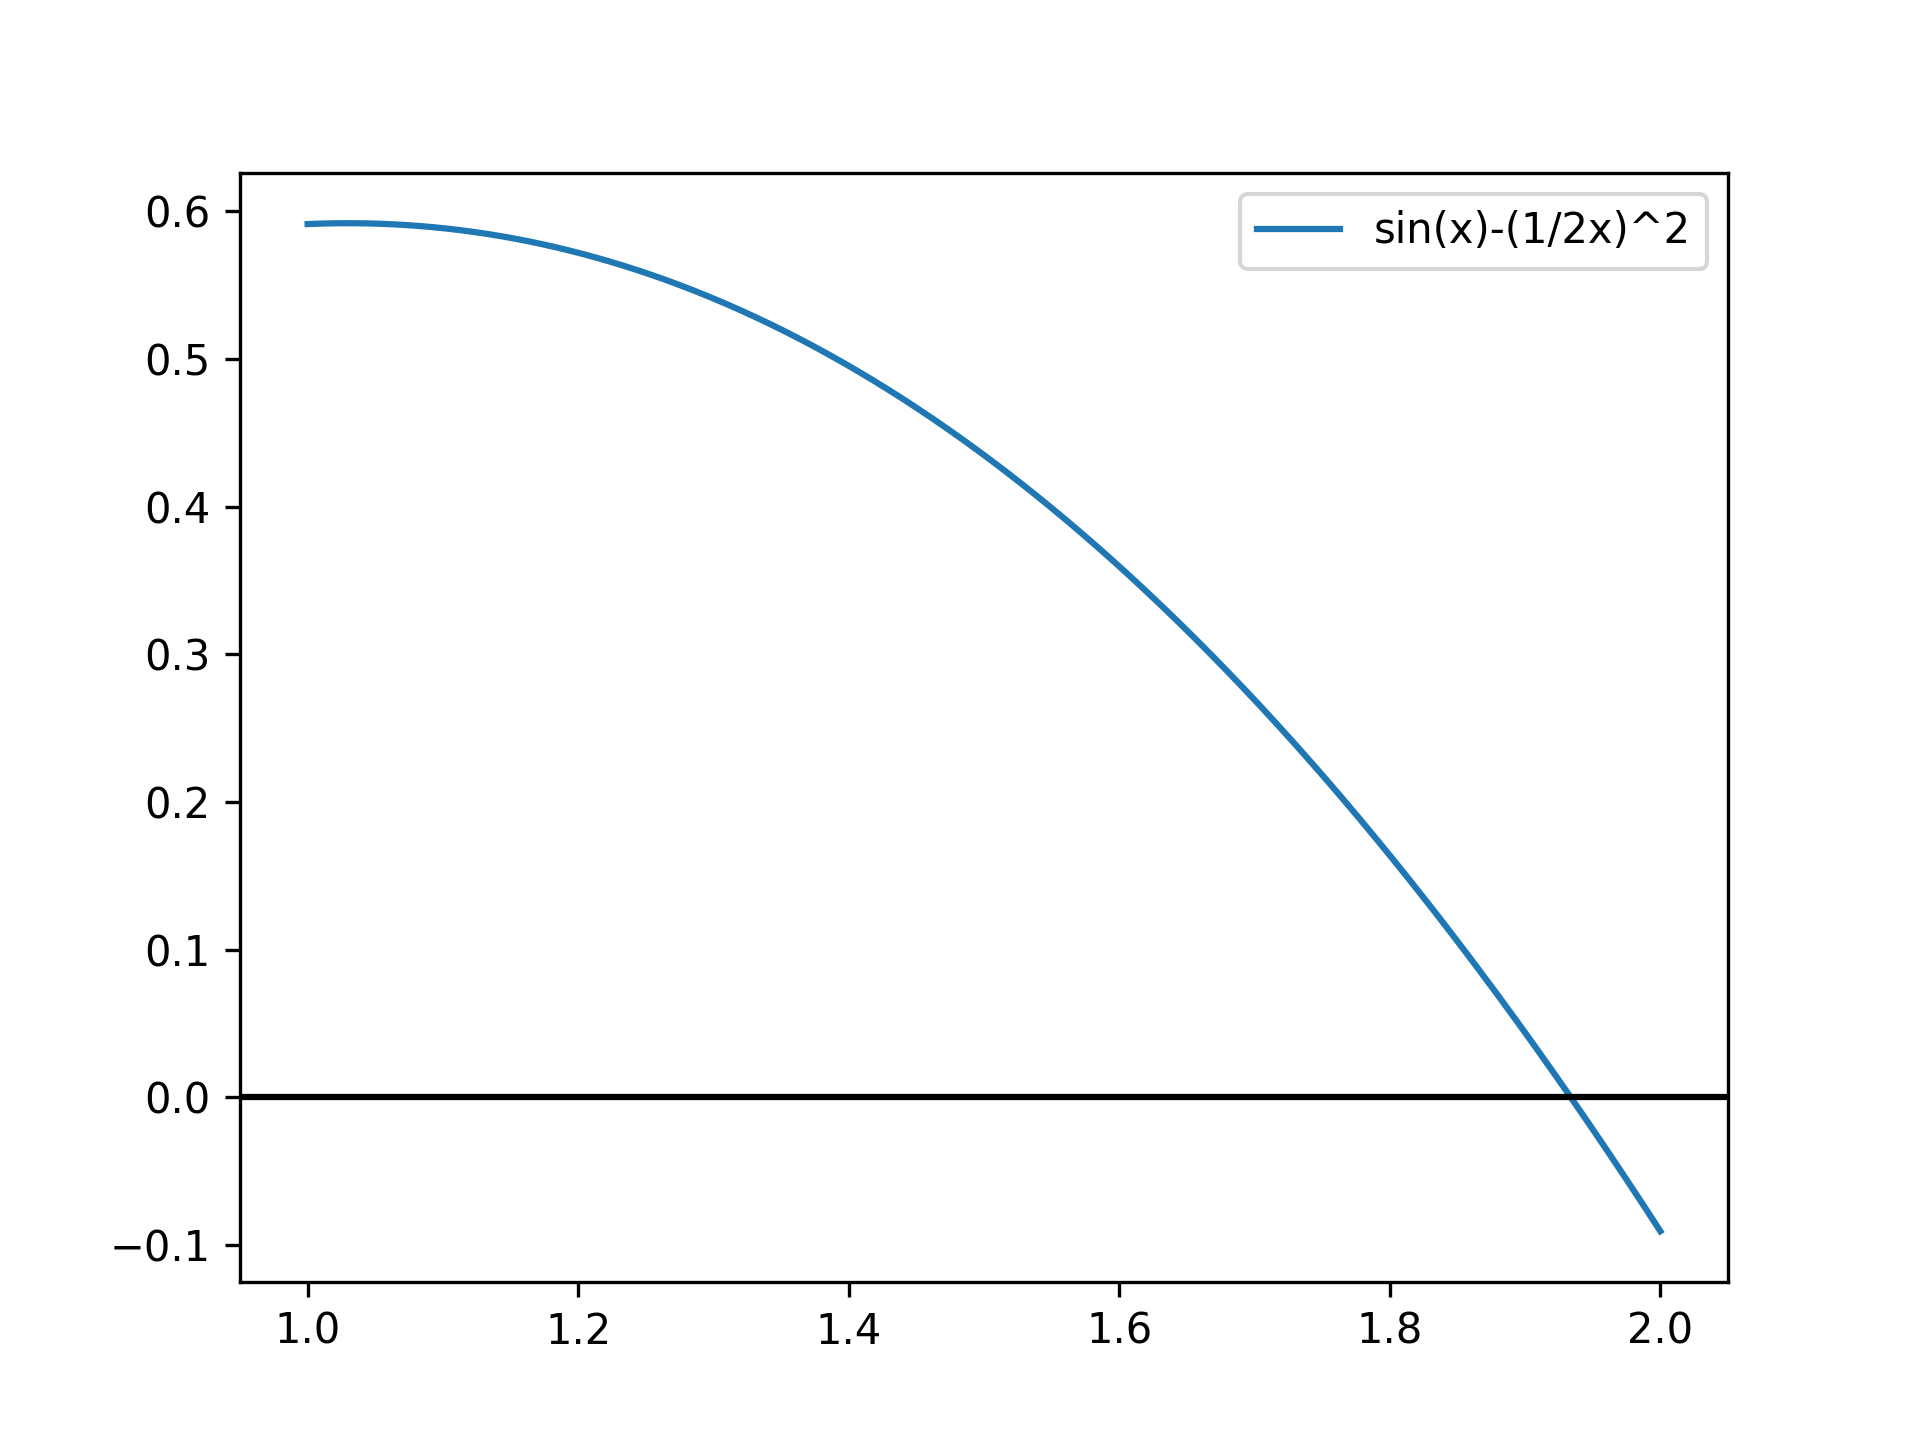
\includegraphics[width=0.6\linewidth]{zad4_plot.png}
  \caption{Wykres w pyplot na przedziale $[1, 2]$}\label{fig:figure1}
\end{figure}

\textbf{Wyniki:}\\
\begin{table}[h!]
	\centering
    \label{tab:table1}
    \begin{tabular}{c|c|c|c|c}
    		Metoda & Miejsce zerowe $x_0$ & $f(x_0)$ & Liczba iteracji & Kod błędu \\
 		\hline
 		\hline
    		bisekcja & 1.9337539672851562 & -2.7027680138402843e-7 & 16 & 0\\
      	\hline
      	stycznych & 1.933753779789742 & -2.2423316314856834e-8 & 4 & 0\\
      	\hline
      	siecznych & 1.933753644474301 & 1.564525129449379e-7 & 4 & 0\\
		\hline
    \end{tabular}
\end{table}

\noindent \textbf{Wnioski:}\\
Patrząc na wyniki możemy dostrzec iż wszystkie metody wykonały obliczenia poprawnie i nie zwróciły błędu. Najwydajniejsze okazały się metody siecznych i stycznych, co jest zgodne z oczekiwaniami. Metody te mają większą zbieżność od metody bisekcji i wykonały obliczenia w 4 razy mniejszej liczbie iteracji.



\section{Zadanie 5}
Celem zadania 5 jest znalezienie za pomocą metody bisekcji wartości zmiennej $x$, dla której przecinają się wykresy funkcji $y_1=3x$ i $y_2=e^x$. Wymagane dokładności obliczeń wynoszą: $\delta=10^{-4}$, $\epsilon=10^{-4}$.
Aby znaleźć wartość zmiennej $x$ porównujemy podane funkcje, dzięki czemu otrzymujemy równanie:
\begin{equation*}
3x=e^x
\end{equation*}
Zatem będziemy szukać miejsc zerowych funkcji:
\begin{equation*}
f(x)=3x-e^x
\end{equation*}

\begin{figure}[!h]
\minipage{0.49\textwidth}
  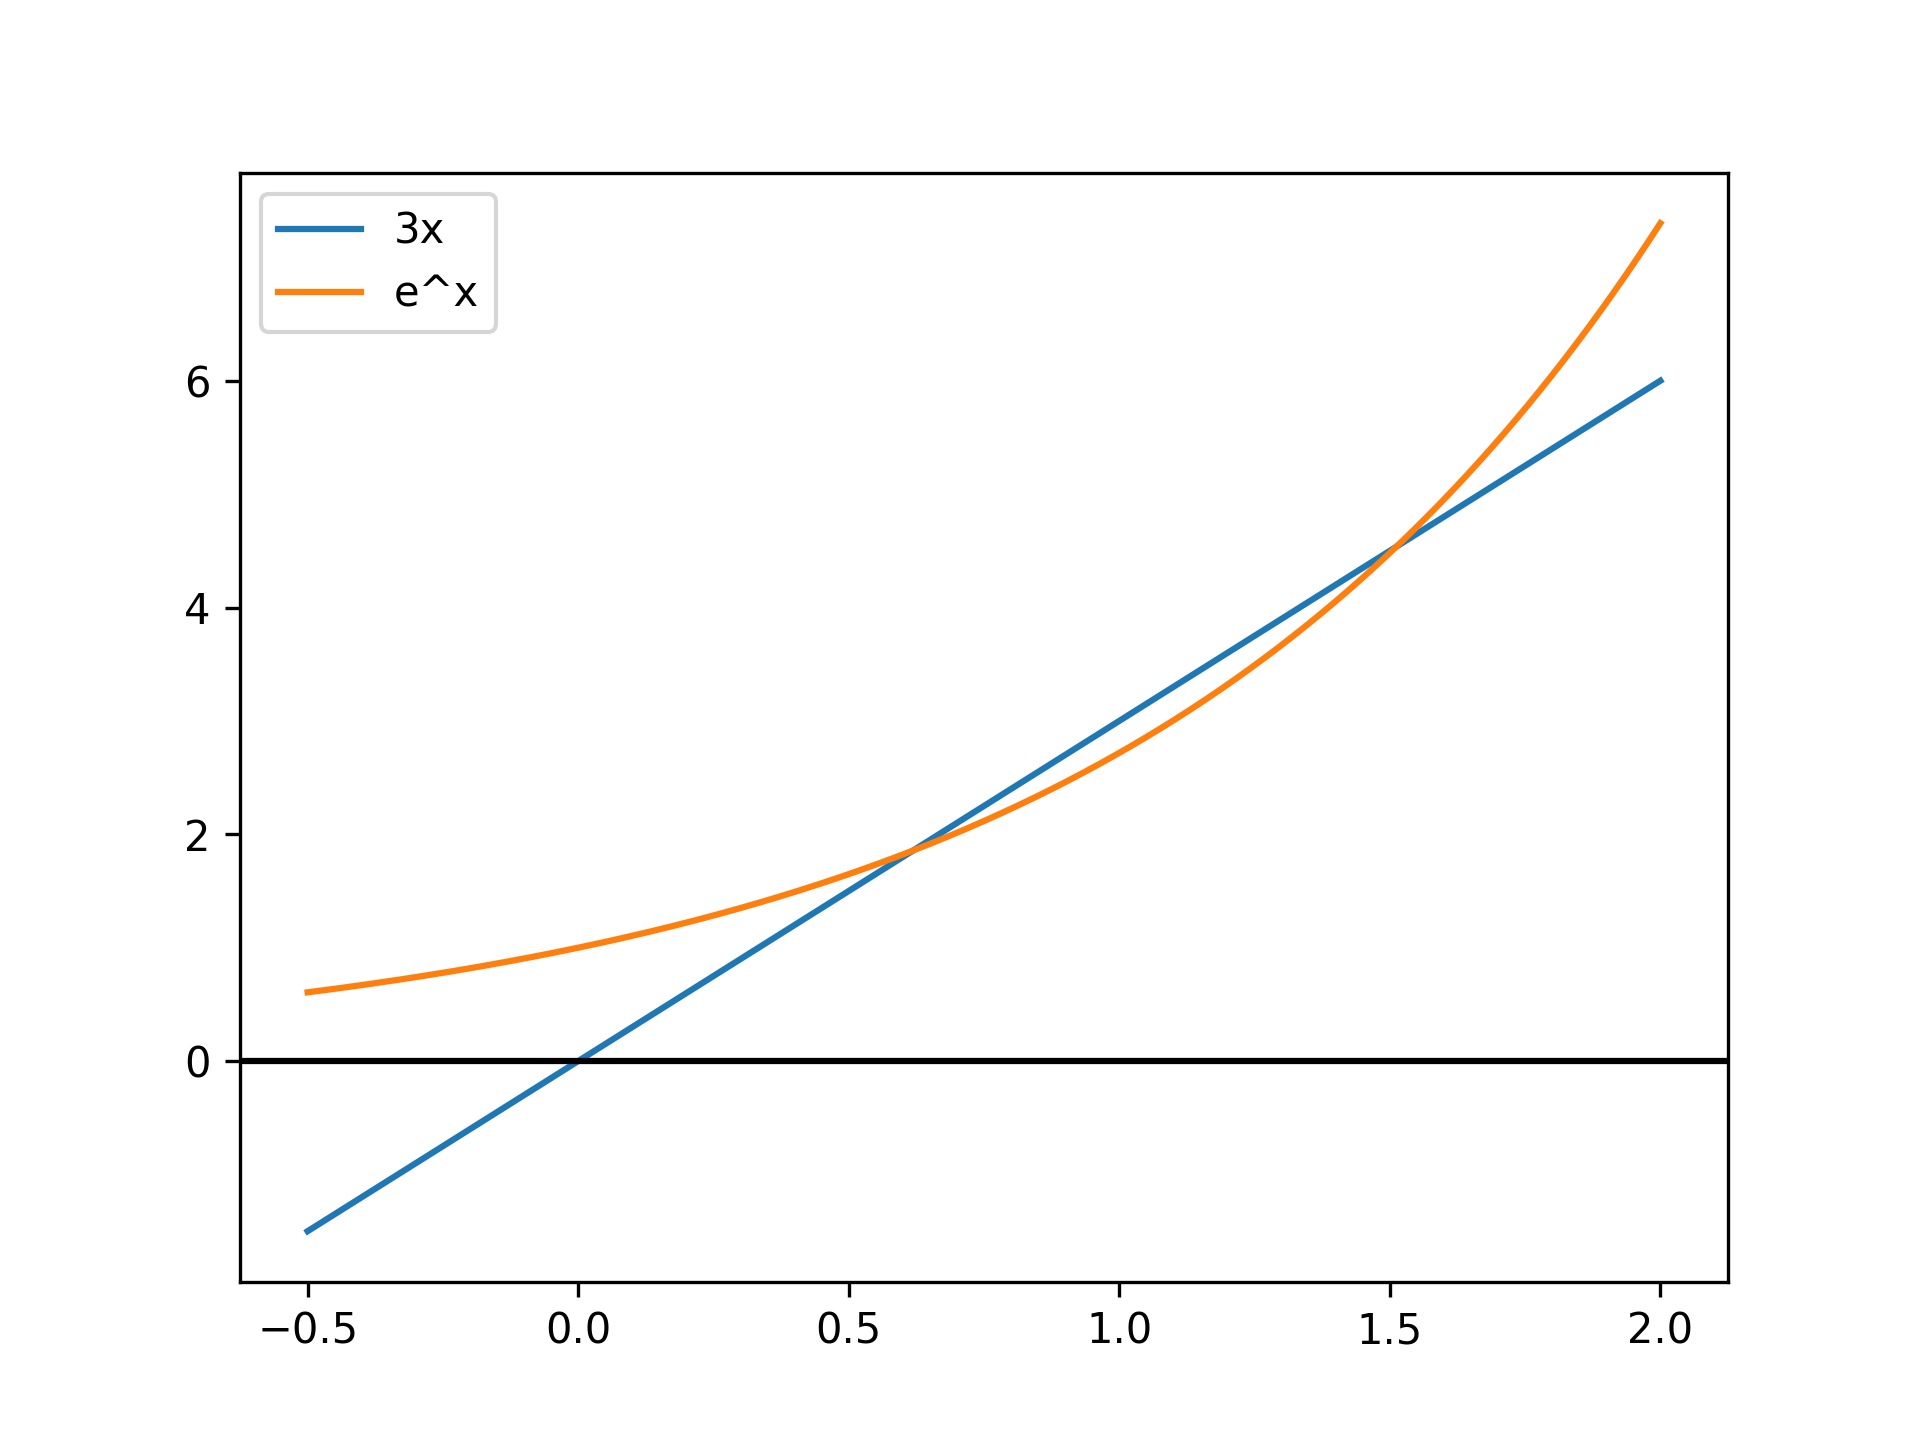
\includegraphics[width=\linewidth]{zad5_a_plot.png}
  \caption{Wykres w pyplot dla $y_1$ i $y_2$}\label{fig:figure1}
\endminipage\hfill
\minipage{0.49\textwidth}
  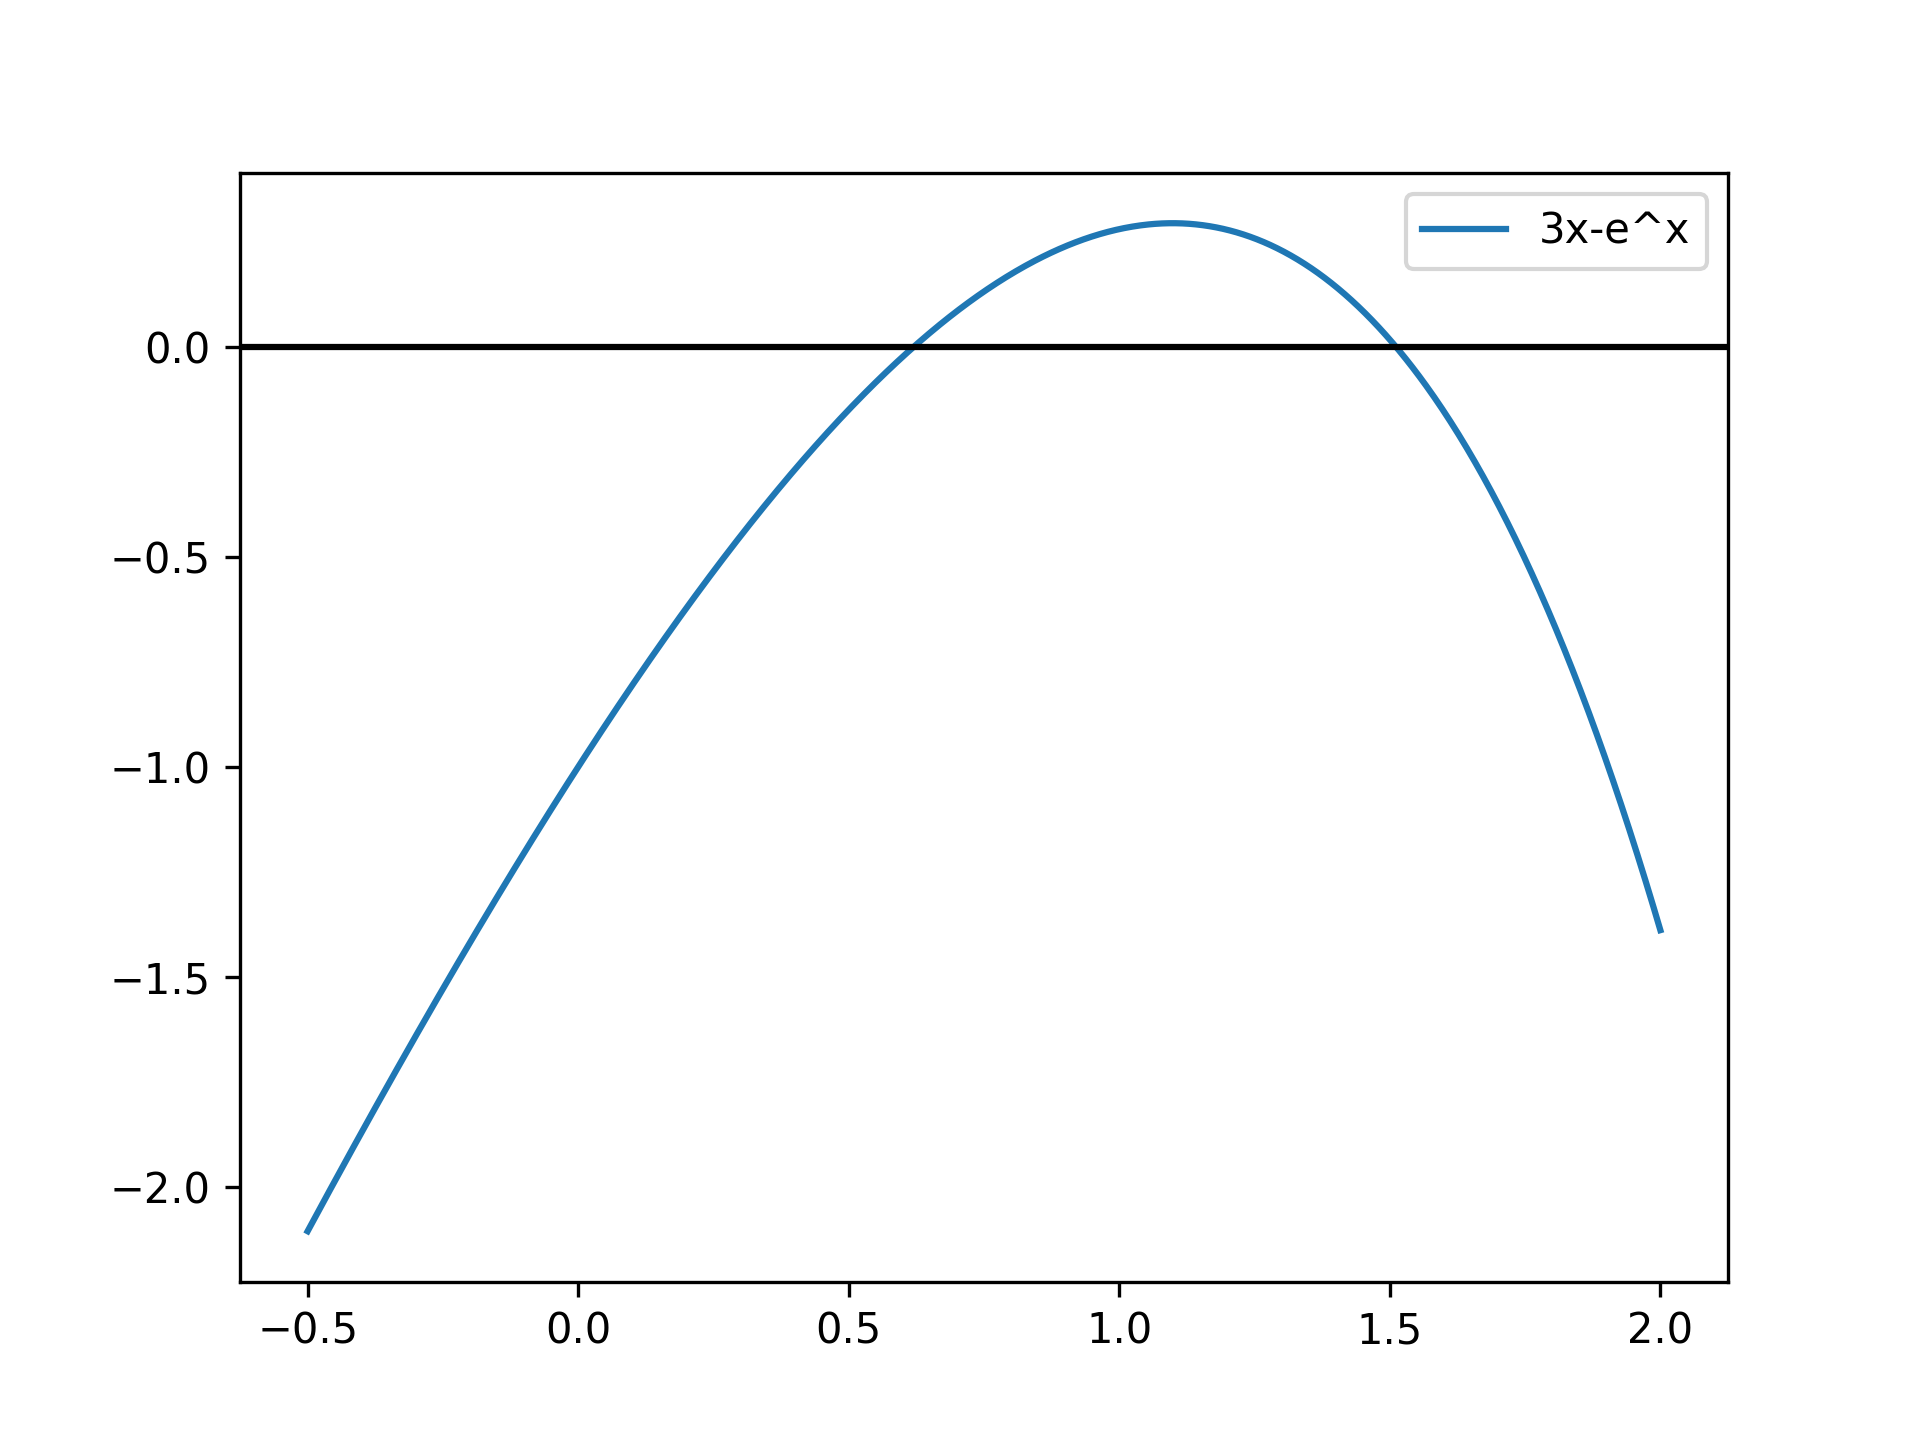
\includegraphics[width=\linewidth]{zad5_b_plot.png}
  \caption{Wykres w pyplot dla $f(x)$}\label{fig:figure2}
\endminipage
\end{figure}

Po wstępnej analizie funkcji można zobaczyć, iż funkcja ma dwa miejsca zerowe. Jako przedziały początkowe dla metody bisekcji wybrałem: $[0.5, 1.0]$ oraz $[1.0, 2.0]$
\\
\\
\noindent \textbf{Wyniki:}\\
Wyniki przedstawia następująca tabela:
\begin{table}[h!]
	\centering
    \label{tab:table2}
    \begin{tabular}{c|c|c|c}
		Miejsce zerowe $x_0$ & $f(x_0)$ & Liczba iteracji & Kod błędu \\
 		\hline
 		\hline
		0.619140625 & 9.066320343276146e-5 & 8 & 0\\
		\hline
		1.5120849609375 & 7.618578602741621e-5 & 13 & 0\\
		\hline
    \end{tabular}
\end{table}
\\
\\
\noindent \textbf{Wnioski:}\\
Algorytm obliczył poszukiwane miejsca zerowe oraz nie zwrócił błędu. Oznacza to że wybraliśmy odpowiednie przedziały. W zadaniu tym główną trudność sprawiało właśnie dobranie odpowiednich przedziałów. W celu znalezienia ich posłużyłem się wykresem funkcji, jednak w przypadku braku dostępu do tego narzędzia musielibyśmy wykonać większą liczbę prób.
\section{Zadanie 6}


\end{document}